
\chapter{ಅಧ್ಯಾಯ ೯: ಝೀಲಮ್​ ಬಳಿಯ ಶತಪಥ ಹಾಗೂ ಮಾತುಕಥೆ}

ವ್ಯಕ್ತಿಗಳು: ಸ್ವಾಮಿ ವಿವೇಕಾನಂದರು, ಗುರುಭಾಯಿಗಳು, ಧೀರಮಾತಾ, ಜಯಾ ಎಂಬ ಹೆಸರಿನವಳು ಮತ್ತು ಸೋದರಿ ನಿವೇದಿತಾಳನ್ನೊಳಗೊಂಡ ಯೂರೋಪಿಯನ್ ಶಿಷ್ಯರುಗಳ ಮತ್ತು ಅತಿಥಿಗಳ ಗುಂಪು.

ಸ್ಥಳ: ಕಾಶ್ಮೀರ.

ಕಾಲ: ೧೮೯೮ರ ಜುಲೈ ೨೦ರಿಂದ ೨೯ರ ವರೆಗೆ.

ಜುಲೈ ೨೦.

ಈ ಹೊತ್ತು ಬೆಳಗ್ಗೆ ನದಿಯು ತಿಳಿಯಾಗಿ, ಅಷ್ಟೊಂದು ಆಳವಿಲ್ಲದಿದ್ದರೂ ವಿಶಾಲ ವಾಗಿತ್ತು. ನಮ್ಮಲ್ಲಿ ಇಬ್ಬರು ಸ್ವಾಮಿಗಳೊಂದಿಗೆ ಹೊಲಗಳ ನಡುವೆ ಹಾಗೂ ನದಿಯ ದಡ ದಲ್ಲೇ ಸುಮಾರು ಮೂರು ಮೈಲಿ ನಡೆದೆವು. ಈಜಿಪ್ಟಿನವರಲ್ಲಿ, ಯಹೂದ್ಯರಲ್ಲಿ \enginline{(Semitic),} ಆರ್ಯರಲ್ಲಿ ಇರುವ ಪಾಪದ ಕಲ್ಪನೆಯಿಂದ ಅವರು ಸಂಭಾಷಣೆಯನ್ನು ಆರಂಭಿಸಿದರು. ವೇದಗಳಲ್ಲಿ ಅದು ಒಂದಿನಿತು ಕಾಣುವುದಾದರೂ, ಬೇಗನೆ ಹೊರಟು ಹೋಗುತ್ತದೆ. ಅನಿಷ್ಟ ಪಿಶಾಚಿಗೆ ಅಲ್ಲಿ ಸಿಟ್ಟಿನ ಅಧಿದೇವತೆ ಎಂದು ಮನ್ನಣೆ ಕೊಡ ಲಾಗಿದೆ. ಅನಂತರ, ಬೌದ್ಧರಲ್ಲಿ ಅದು ಕಾಮದ ದೇವತೆ ಮಾರನಾಗುತ್ತದೆ; ಬುದ್ಧನಿಗೆ ಕೊಡಲಾದ ಅತ್ಯಂತ ಪ್ರೀತಿಯ ಬಿರುದೇ “ಮಾರನನ್ನು ಜಯಿಸಿದವನು” ಎಂಬುದು. (ಇಲ್ಲಿ ಸ್ವಾಮಿಗಳು ನಾಲ್ಕು ವರ್ಷದ ಬಾಲಕನಂತೆ ಕಂಠಪಾಠ ಒಪ್ಪಿಸುತ್ತಿದ್ದ ಅಮರ ಕೋಶವೆಂಬ ಸಂಸ್ಕೃತ ನಿಘಂಟನ್ನು ನೋಡಬಹುದು!) ಆದರೆ ಸೈತಾನ ಬೈಬಲ್ನಲ್ಲಿ ದೇವದೂಷಕನಾಗಿರುವಂತೆ ಹಿಂದೂ ಶಾಸ್ತ್ರಗ್ರಂಥಗಳಲ್ಲಿ ಸಿಟ್ಟಿನ ಅಧಿದೇವತೆ ಸೃಷ್ಟಿಯನ್ನು ಒಡೆಯುವುದಿಲ್ಲ. ಅವನು ಪ್ರತಿನಿಧಿಸುವುದು ಅಪವಿತ್ರತೆಯನ್ನೇ ಹೊರತು ದ್ವೈತವನ್ನಲ್ಲ.

ಹಳೆಯ ಕೆಲವು ಧರ್ಮಗಳಲ್ಲಿ ಜರತುಷ್ಟ್ರನು ಒಬ್ಬ ಸುಧಾರಕನಾಗಿ ಕಾಣಿಸಿ ಕೊಳ್ಳುತ್ತಾನೆ. ಅವನೊಡನಿದ್ದ ಆರ್ಮುಜ್ಡ ಅಹ್ರಿಮಾನ್ರೂ ಸಹ ಪರಮ ಎನ್ನಿಸಿಕೊಳ್ಳು ವುದಿಲ್ಲ; ಬದಲಿಗೆ ಪರಮವೆಂಬುದರ ಪ್ರತೀಕವಾಗುತ್ತಾರೆ. ಆ ಹಳೆಯ ಧರ್ಮ ವೇದಾಂತದ್ದಾಗಿರಬೇಕು. ಹೀಗೆ, ಈಜಿಪ್ಟಿನವರೂ ಯಹೂದಿಗಳೂ \enginline{(Semites)} ಪಾಪದ ಕಲ್ಪನೆಗೆ ಅಂಟಿಕೊಂಡೇ ಮುನ್ನಡೆದರೆ, ಆರ್ಯರು ಗ್ರೀಕರಾಗಿ, ಭಾರತೀಯರಾಗಿ, ಅದನ್ನು ಬೇಗನೆ ಕಳೆದುಕೊಳ್ಳುತ್ತಾರೆ. ಭಾರತದಲ್ಲಿ ಋಜುತ್ವ ಹಾಗೂ ಪಾಪಗಳು, ಎರಡನ್ನೂ ಮೀರಿ ಹೋಗಿ ವಿದ್ಯಾ ಮತ್ತು ಅವಿದ್ಯಾ ಎಂದೆನ್ನಿಸಿಕೊಳ್ಳುತ್ತವೆ. ಆರ್ಯರಲ್ಲೇ ಪರ್ಷಿಯನ್ನರು ಮತ್ತು ಯೂರೋಪಿಯನ್ನರು ಯಹೂದಿಗಳಿಂದ ಕಲ್ಪನೆಗಳನ್ನು ಪಡೆ ಯುತ್ತಾರೆ; ಹಾಗೆ ಪಾಪದ ಕಲ್ಪನೆಯೂ ಬರುತ್ತದೆ\footnote{1. ಅಂದು ಈ ಭಾಷಣವನ್ನು ಕೇಳಿದವರಲ್ಲಿ ಒಬ್ಬರಿಗೆ ಆ ನಂತರ ಸ್ವಾಮಿಗಳ ಜ್ಞಾನದ ನಿಷ್ಕೃಷ್ಟತೆ ಮತ್ತು ವೈಶಾಲ್ಯಗಳನ್ನರಿಯುವ ಅಚ್ಚರಿಯ ಅವಕಾಶವೊಂದು ಎದುರಾಯಿತು - ಇಬ್ಬರು ಪಾರ್ಸಿಗಳು ಸಂತೋಷದಿಂದ ಸ್ವಾಮಿಗಳ ಪದತಲದಲ್ಲಿ ಕುಳಿತು ತಮ್ಮದೇ ಧಾರ್ಮಿಕ ಕಲ್ಪನೆಗಳ ಇತಿಹಾಸವನ್ನು ಅವರಿಂದ ಕಲಿಯುವುದನ್ನು ಅವಳು ಪ್ರತ್ಯಕ್ಷವಾಗಿ ನೋಡಿದಳು. -ನಿವೇದಿತಾ.}.

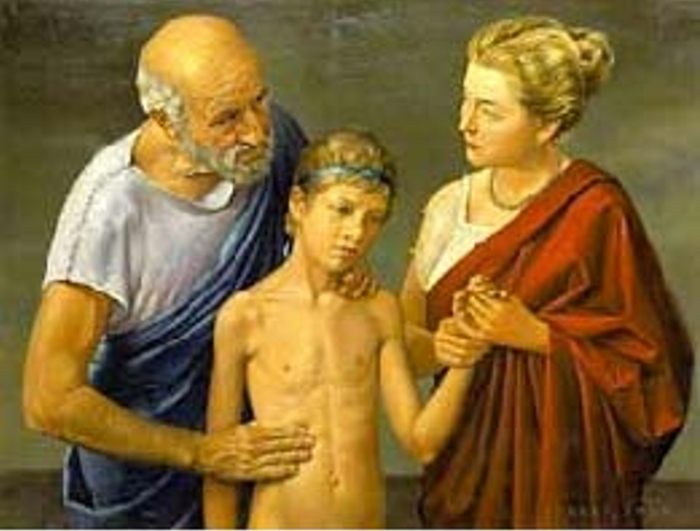
\includegraphics{images/005.jpg}
ಅನಂತರ ಮಾತುಕತೆ ಬೇರೆಕಡೆ ಹೊರಳಿತು - ಯಾವಾಗಲೂ ಅದು ಆಗಬೇಕಾದದ್ದೇ ಹಾಗೆ - ದೇಶದ ಹಾಗೂ ಭವಿಷ್ಯದ ಪ್ರಶ್ನೆಗಳ ಕಡೆಗೆ ಹೊರಳಿತು. ಜನರಿಗೆ ಶಕ್ತಿಯನ್ನು ಒದಗಿಸಬೇಕಾದರೆ ಅವರಿಗೆ ಯಾವ ಕಲ್ಪನೆಯನ್ನು ಕೊಡಬೇಕು? ಅವರು ಬೆಳೆದುಬರುವ ಮಾರ್ಗವೇ ಒಂದು ರೀತಿಯಾಗಿರುತ್ತದೆ - ಅದನ್ನು \textbf{ಅ} ಎಂದಿಟ್ಟುಕೊಳ್ಳೋಣ. ಹೊಸದಾಗಿ ಕೊಡಲ್ಪಡುವ ಬಲವು ಅದಕ್ಕೆ ಪೂರಕವಾಗಿರು ವಂತಹ
 \textbf{ಬ} ಎಂಬುದಾಗಿ ಇಟ್ಟುಕೊಳ್ಳೋಣವೆ? ಆಗ ಅವರು ಅಭಿವೃದ್ಧಿ ಹೊಂದುತ್ತ ಬರುವ ದಾರಿ ಇವೆರಡರ ನಡುವಣ \textbf{ಕ} ಆಗಿರುತ್ತದೆ - ಕೇವಲ ಒಂದು ಜ್ಯಾಮಿತೀಯ ಬದಲಾವಣೆಯ ಹಾಗೆ. ಆದರೆ ಅದು ಹಾಗೆ ಆಗಿ ಬರಲಿಲ್ಲ.

ರಾಷ್ಟ್ರೀಯ ಜೀವನವೆಂದರೆ ಅದೊಂದು ಜೀವಂತಿಕೆಯ ಬಲಗಳ ಪ್ರಶ್ನೆ. ನಾವು ಆ ಜೀವನಪ್ರವಾಹದೊಂದಿಗೆ ಸೇರಿ ಅದನ್ನು ಬಲಪಡಿಸಬೇಕು; ಉಳಿದೆಲ್ಲವನ್ನೂ ಅದೇ ಮಾಡುವಂತೆ ಬಿಡಬೇಕು. ಬುದ್ಧ ತ್ಯಾಗವನ್ನು ಬೋಧಿಸಿದನು; ಭಾರತವು ಕಿವಿಗೊಟ್ಟು ಕೇಳಿತು. ಆದರೂ, ಒಂದು ಸಾವಿರ ವರ್ಷದೊಳಗೆ ಅದು ರಾಷ್ಟ್ರೀಯ ಅಭಿವೃದ್ಧಿಯ ಪರಾಕಾಷ್ಠೆಯನ್ನು ತಲುಪಿತು. ಭಾರತದಲ್ಲಿ ರಾಷ್ಟ್ರೀಯ ಜೀವನದ ಮೂಲವೇ ತ್ಯಾಗ. ಅದರ ಉನ್ನತಾದರ್ಶಗಳೇ ಸೇವೆ ಮತ್ತು ಮುಕ್ತಿ. ಹಿಂದೂ ಕುಟುಂಬದಲ್ಲಿ ತಾಯಿಯಾದ ವಳು ಊಟ ಮಾಡುವುದು ಕೊನೆಯಲ್ಲಿ. ಮದುವೆ ಎನ್ನುವುದು ವೈಯಕ್ತಿಕ ಸುಖಕ್ಕಾಗಿ ಅಲ್ಲ, ಜಾತಿಯ ಹಾಗೂ ಜನಾಂಗದ ಹಿತಕ್ಕಾಗಿ. ಸಮಸ್ಯೆಗಳು ಪರಿಹಾರವಾಗದ ಕೆಲವು ಪ್ರಯೋಗಗಳನ್ನು ನವಯುಗದ ಕೆಲವು ಸುಧಾರಕರುಗಳು ಕೈಕೊಂಡಿರುವರು; “ಇಡಿಯ ಜನಾಂಗವೇ ಇವರ ಈ ತ್ಯಾಗಗಳ ಮೇಲೆ ನಡೆದು ಬರಬೇಕಾಗಿದೆ.”

ಅನಂತರ, ಸಂಭಾಷಣೆಯ ದಿಕ್ಕು ಮತ್ತೊಮ್ಮೆ ಬದಲಾಯಿತು; ಹಾಸ್ಯರಸಾಸ್ವದನೆ ತಾನೇ ತಾನಾಯಿತು - ನಗೆಚಾಟುಗಳು, ಕಥೆಗಳು ಬರತೊಡಗಿದವು. ನಾವುಗಳೆಲ್ಲ ನಗುತ್ತ, ಕೇಳುತ್ತ ಇದ್ದಂತೆಯೇ ದೋಣಿಗಳು ಬಂದವು; ದಿನದ ಮಟ್ಟಿಗೆ ಮಾತುಕಥೆ ಕೊನೆಗೊಂಡಿತು.

ಆ ದಿನ ಮಧ್ಯಾಹ್ನವಿಡೀ ಮತ್ತು ರಾತ್ರಿ ಸ್ವಾಮಿಗಳು ಅಸ್ವಸ್ಥರಾಗಿ ತಮ್ಮ ದೋಣಿಯಲ್ಲೇ ಇದ್ದುಬಿಟ್ಟರು. ಆದರೆ ಮಾರನೆಯ ದಿನ, ನಾವುಗಳು ಬಿಜ್ಬೇಹಾರ ದೇವಾಲಯಕ್ಕೆ ಬಂದು ತಲುಪಿದೊಡನೆ - ಅದಾಗಲೇ ಅಮರನಾಥ ಯಾತ್ರಿಕರೊಂದಿಗೆ ಗುಂಪುಗೂಡಿದ್ದೆವು - ಅವರು ಸ್ವಲ್ಪ ಕಾಲ ನಮ್ಮೊಂದಿಗೆ ಬಂದು ಸೇರುವಂತಾದರು. ಅವರು ತಮ್ಮ ಬಗ್ಗೆ ತಾವೇ ಹೇಳಿಕೊಳ್ಳುತ್ತಿದ್ದಂತೆ, “ಮಲಗುವುದೂ ಬೇಗ, ಏಳುವುದೂ ಬೇಗ” ಎಂಬುದೇ ಅವರ ವೈಶಿಷ್ಟ್ಯವಾಗಿದ್ದಿತು. ಅದಾದ ಮೇಲೆ ದಿನವಿಡೀ ಅವರು ನಮ್ಮ ಜೊತೆಗೇ ಇದ್ದರು; ಮಧ್ಯಾಹ್ನದ ಹೊತ್ತಿಗೆ ನಾವು ಇಸ್ಲಾಮಾಬಾದ್ ತಲುಪಿದೆವು...

ಆ ದಿನ ಸಂಜೆಗತ್ತಲಿನಲ್ಲಿ ಸೇಬಿನ ಮರಗಳಡಿ ಇದ್ದ ಸಣ್ಣದೊಂದು ಗುಂಪಿಗೆ ಒಬ್ಬರು ಬಂದು ಸೇರುತ್ತಲೂ, ಅಪರೂಪವೆನ್ನಿಸುವಂಥ ಘಟನೆಯೊಂದರಲ್ಲಿ ಸ್ವಾಮಿಗಳು ಧೀರ ಮಾತಾ ಹಾಗೂ ಜಯಾಳೊಂದಿಗೆ ಆಪ್ತಸಂಭಾಷಣೆಯಲ್ಲಿದ್ದುದನ್ನು ಕಾಣುವಂತಾ ಯಿತು. ಅವರು ತಮ್ಮ ಕೈಯಲ್ಲಿ ಎರಡು ದುಂಡುಕಲ್ಲುಗಳನ್ನು ಹಿಡಿದು, ಹೇಗೆ ತಾವು ಆರೋಗ್ಯವಾಗಿರುವಾಗ ತಮ್ಮ ಮನಸ್ಸು ಅಲ್ಲಿ-ಇಲ್ಲಿ ಹರಿದಾಡಬಹುದು, ಹೇಗೆ ತಮ್ಮ ಇಚ್ಛಾಶಕ್ತಿ ಸ್ವಲ್ಪ ತಗ್ಗಿದಂತೆ ಅನ್ನಿಸಬಹುದು; ಆದರೆ ನೋವಿನ ಅಥವಾ ಕಾಹಿಲೆಯ ಅಲ್ಪ ಸಂಸ್ಪರ್ಶವಾದರೂ ಸಾಕು, ಮೃತ್ಯುವಿನ ಕ್ಷಣಿಕದರ್ಶನವಾದರೂ ಸಾಕು, (ಕೈಯ ಲ್ಲಿದ್ದ ಎರಡು ಕಲ್ಲುಗಳನ್ನು ಪರಸ್ಪರ ಸಂಘಟ್ಟಿಸುತ್ತ) “ನಾನು ಅಷ್ಟೊಂದು ಕಠಿಣನಾಗಿ ಬಿಡುತ್ತೇನೆ, ಏಕೆಂದರೆ ನಾನು ಭಗವಂತನ ಪಾದಾರವಿಂದಗಳನ್ನು ಮುಟ್ಟಿರುವೆ” ಎಂದು ಹೇಳುತ್ತಿದ್ದರು.

ಈ ಶಾಂತಸ್ವಭಾವಕ್ಕೆ ಸಂಬಂಧಿಸಿದಂತೆ ನೆನಪಾಗುವುದು ಇಂಗ್ಲೆಂಡಿನ ಹೊಲಗಳಲ್ಲಿ ಸ್ವಾಮಿಗಳು, ಒಬ್ಬ ಆಂಗ್ಲ ಮತ್ತು ಒಬ್ಬ ಮಹಿಳೆ ನಡೆದಾಡುತ್ತಿದ್ದಾಗಿನ ಒಂದು ಪ್ರಸಂಗ. ಈ ಮೂವರನ್ನೂ ಒಂದು ಕೋಪೋದ್ರಿಕ್ತ ಗೂಳಿ ಅಟ್ಟಿಸಿಕೊಂಡು ಬಂದಿತು. ಆಂಗ್ಲನು ಹಿಂದುಮುಂದು ನೋಡದೆ ಓಡಿ ಗುಡ್ಡದ ಇನ್ನೊಂದು ಭಾಗಕ್ಕೆ ಹೋಗಿ ಸೇರಿ ತಪ್ಪಿಸಿ ಕೊಂಡುಬಿಟ್ಟ. ಮಹಿಳೆ ತನಗೆ ಸಾಧ್ಯವಿರುವಷ್ಟೂ ಓಡಿದಳು; ಮುಂದೆ ಓಡಲಾರದೆ ಮುಗ್ಗರಿಸಿ ಬಿದ್ದಳು; ಅವಳಿಗೆ ಏಳುವುದಕ್ಕೆ ಸಾಧ್ಯವಾಗಲಿಲ್ಲ. ಇದನ್ನು ನೋಡಿದ ಸ್ವಾಮಿಗಳು, ಅವಳಿಗೆ ನೆರವನ್ನೂ ನೀಡಲಾಗದೆ, “ಒಹೋ, ಇದೇ ಕೊನೆ ಎಂದು ಕಾಣುತ್ತದೆ” ಎಂದು ಯೋಚಿಸುತ್ತ, ಅವಳ ಮುಂದೆ ಕೈಮುಗಿದು ನಿಂತುಕೊಂಡರು. ಆ ನಂತರ ಅವರು ಹೇಳಿದಂತೆ, ಗೂಳಿ ತಮ್ಮನ್ನು ಎಷ್ಟು ದೂರಕ್ಕೆ ಎತ್ತಿ ಒಗೆಯಬಲ್ಲುದು ಎಂದು ಅವರ ಮನಸ್ಸು ಆಗ ಗಣಿತದ ಲೆಕ್ಕಾಚಾರ ಹಾಕುತ್ತಿದ್ದಿತಂತೆ. ಆದರೆ ಓಡಿ ಬರುತ್ತಿದ್ದ ಗೂಳಿ ಇದ್ದಕ್ಕಿದ್ದಂತೆ ಸ್ವಲ್ಪ ದೂರದಲ್ಲೇ ನಿಂತು, ತಲೆ ಎತ್ತಿ ನೋಡಿ, ಮಂಕು ಬಡಿದಂತೆ ಸುಮ್ಮನೆ ಹಿಂದಿರುಗಿತಂತೆ.

ಸ್ವಾಮಿಜಿಯವರು ಈ ಘಟನೆಗಳ ಬಗ್ಗೆ ಎಂದೂ ಯೋಚಿಸುತ್ತಿರಲಿಲ್ಲ. ಇಂತಹುದೇ ಧೈರ್ಯ ಅವರ ನವತಾರುಣ್ಯದಲ್ಲಿಯೂ ಒಮ್ಮೆ ಅಭಿವ್ಯಕ್ತವಾಗಿತ್ತು. ಗಾಡಿಗೆ ಕಟ್ಟಿದ್ದ ಕುದುರೆಯೊಂದು ಹುಚ್ಚೆದ್ದು ಓಡತೊಡಗಿದಾಗ, ಓಡುತ್ತ ಬಂದ ಕುದುರೆಯ ಮೇಲೇರಿ, ಕಲ್ಕತ್ತದ ಬೀದಿಯಲ್ಲಿ ಅದನ್ನು ನಿಯಂತ್ರಿಸಿ, ಹಿಂದೆ ಗಾಡಿಯಲ್ಲಿದ್ದ ಸ್ತ್ರೀ ಯೊಬ್ಬರ ಜೀವವನ್ನು ಅವರು ಕಾಪಾಡಿದ್ದರು.

ಹೀಗೆಯೇ ಒಂದೆರಡು ಗಂಟೆಗಳ ಕಾಲ ಮಾತು ಸಾಗಿತ್ತು - ಮರಗಳ ಕೆಳಗೆ ಹುಲ್ಲಿನ ಮೇಲೆ ನಾವು ಕುಳಿತಿದ್ದಂತೆಯೇ; ಅರೆವಾಸಿ ಗಂಭೀರವಾಗಿ, ಅರೆವಾಸಿ ಹಾಸ್ಯವಾಗಿ. ವೃಂದಾವನದ ಮಂಗಗಳು ಅಲ್ಲಿಗೆ ಬರುವ ಮನುಷ್ಯರನ್ನು ಗೋಳಾಡಿಸುವ ಅನೇಕ ಚೇಷ್ಟೆಗಳನ್ನು ಕೇಳಿದೆವು. ಅವರ ಪರಿವ್ರಾಜಕ ಜೀವನದ ಎರಡು ಪ್ರತ್ಯೇಕ ಸಂದರ್ಭಗಳಲ್ಲಿ ಸಹಾಯವು ಬರುವುದರ ಪೂರ್ವಸೂಚನೆ ದೊರಕಿದ, ನಂತರ ಅದು ನಿಜವಾದ ಕಥೆಗಳನ್ನು ಕೇಳಿ ತಿಳಿದೆವು. ಇವುಗಳಲ್ಲಿ ಒಂದು ನನಗೆ ನೆನಪಿದೆ. ಇದು ಬಹುಶಃ ಸ್ವಾಮಿಗಳು ತಾವು ಏನನ್ನೂ ಬೇಡುವುದಿಲ್ಲವೆಂಬ ವ್ರತದಲ್ಲಿದ್ದಾಗ ನಡೆದಿರಬಹುದು. ಒಮ್ಮೆ ಅವರು ಅನೇಕ ದಿನ (ಬಹುಶಃ ಐದು ದಿನಗಳು) ಆಹಾರವಿಲ್ಲದೆ ಇರಬೇಕಾಯಿತು. ಇದ್ದಕ್ಕಿದ್ದಂತೆ, ಶಕ್ತಿಯೆಲ್ಲವೂ ಉಡುಗಿ ಹೋಗಿ ಇನ್ನೇನು ಸಾವು ಸಮೀಪಿಸಿದೆಯೆನ್ನು ವಂತಹ ಸ್ಥಿತಿಯಲ್ಲಿ ರೈಲ್ವೆ ನಿಲ್ದಾಣವೊಂದರಲ್ಲಿ ಬಿದ್ದುಕೊಂಡಿದ್ದಾಗ, ತಾವು ಎದ್ದು ಹೊರಗೆ ಇಂಥದೊಂದು ರಸ್ತೆಯಲ್ಲಿ ನಡೆದರೆ ಅಲ್ಲಿ ತಮಗೆ ಸಹಾಯ ತರುತ್ತಿರುವ ಒಬ್ಬ ಮನುಷ್ಯ ಸಿಗುತ್ತಾನೆ ಎಂದು ಅವರ ಮನಸ್ಸಿಗೆ ಹೊಳೆಯಿತಂತೆ. ಈ ಹೊಳಹನ್ನು ಅನುಸರಿಸಿ ಅವರು ಹೊರಟಾಗ, ತಟ್ಟೆಯಲ್ಲಿ ಬಡಿಸಿದ ಭೋಜನವನ್ನಿಟ್ಟುಕೊಂಡು ಬರುತ್ತಿರುವ ಒಬ್ಬನ ಭೇಟಿಯಾಯಿತಂತೆ. ಹತ್ತಿರಕ್ಕೆ ಬಂದ ಅವನು ಇವರನ್ನು ದಿಟ್ಟಿಸಿ ನೋಡುತ್ತ “ನಾನು ಯಾರಿಗಾಗಿ ಕಳುಹಿಸಲ್ಪಟ್ಟಿರುವೆನೋ ಅವರು ನೀವೇ ಏನು?” ಎಂದು ವಿಚಾರಿಸಿದನಂತೆ.

ಆಗ ಕೈಗೆ ಕೊಯ್ತದ ಗಾಯ ಮಾಡಿಕೊಂಡ ಮಗುವೊಂದನ್ನು ಯಾರೋ ನಮ್ಮ ಬಳಿಗೆ ಕರೆತಂದರು. ಸ್ವಾಮಿಗಳು ಅದಕ್ಕೆ ತಮಗೆ ಗೊತ್ತಿದ್ದ ಹಳೆಯ ಕಾಲದ ಅಜ್ಜಿ ವೈದ್ಯವನ್ನು ಮಾಡಿದರು- ಗಾಯವನ್ನು ನೀರಿನಿಂದ ತೊಳೆದು, ರಕ್ತಸ್ರಾವವನ್ನು ನಿಲ್ಲಿಸುವುದಕ್ಕೆ ಕ್ಯಾಲಿಕೋ ತುಂಡೊಂದನ್ನು ಸುಟ್ಟ ಬೂದಿಯನ್ನು ಉದುರಿಸಿದರು. ಹಳ್ಳಿಗರಿಗೆಲ್ಲ ಸಮಾಧಾನವಾಯಿತು; ನಮ್ಮ ಸಂಜೆಯ ಹರಟೆಯೂ ಅಲ್ಲಿಗೆ ಮುಕ್ತಾಯವಾಯಿತು.

\textbf{ಜುಲೈ ೨೩.}

ಮಾರನೆಯ ಬೆಳಗ್ಗೆ ನಮ್ಮನ್ನು ಮಾರ್ತಾಂಡ ದೇವಾಲಯದ ಭಗ್ನಾವಶೇಷಗಳ ಕಡೆಗೆ ಕರೆದುಕೊಂಡು ಹೋಗುವುದಕ್ಕೆಂದು ಬಂದು ಸೇರಿದ್ದ ವಿವಿಧ ಕೂಲಿಜನರ ಗುಂಪೊಂದು ಸೇಬಿನ ಮರಗಳ ಕೆಳಗೆ ಅನೇಕ ಗಂಟೆಗಳಿಂದ ಕಾಯುತ್ತಿತ್ತು. ಅದೊಂದು ಅದ್ಭುತವಾದ ಹಳೆಯ ಕಟ್ಟಡ - ದೇವಸ್ಥಾನಕ್ಕಿಂತ ಹೆಚ್ಚಾಗಿ ಕ್ರೈಸ್ತಮಠವನ್ನು ಹೋಲುತ್ತಿದ್ದಂಥದು - ಅಚ್ಚರಿಯ ಸ್ಥಾನದಲ್ಲಿತ್ತು; ಅದು ಸಾಗಿ ಬಂದ ಕಾಲಘಟ್ಟಗಳಿಗನುಗುಣವಾಗಿ ಶಿಲ್ಪ ಶೈಲಿ ಗಳ ಸಮ್ಮಿಶ್ರಣವನ್ನು ಹೊತ್ತು ನಿಂತು ಕುತೂಹಲವನ್ನು ಹೆಚ್ಚಿಸುತ್ತಿತ್ತು... ಪ್ರಾಚ್ಯವೇ ಮೂಲತಃ ಸಂನ್ಯಾಸದ ತವರು ಎಂಬುದನ್ನು ಮತ್ತೆ ಮತ್ತೆ ನೆನಪಿಸುವಂತೆ ಇತ್ತು. ಕ್ಷಣದಲ್ಲಿ ಸ್ವಾಮಿಗಳು ಕಾರ್ಯೋನ್ಮುಖರಾದರು; ಸೂಕ್ಷ್ಮ ಪರಿಶೀಲನೆ, ನಂತರ ಊಹನೆ, ನಂತರ ತೀರ್ಮಾನ, ವಾದಗಳು. ಮಧ್ಯಾಂಗಣದಿಂದ ಗರ್ಭಗುಡಿಯವರೆಗೆ ಇದ್ದ ಕಾರಣೆಯನ್ನು ತೋರಿಸುವರು; ಪಶ್ಚಿ ಮದ ಕಡೆಗೆ ಇದನ್ನು ಮುಸುಕಿದ ಎತ್ತರದ ಎರಡು ಕಮಾನುಗಳಲ್ಲಿನ ತ್ರಿದಳಾಕೃತಿಯ ಅಲಂಕರಣ ಹಾಗೂ ಬೋದಿಗೆ ತೊಲೆಗಳ ನಡುವಣ ಜಾಗದ ಅಲಂಕರಣಗಳನ್ನು ತೋರಿಸುವರು; ರೆಕ್ಕೆ ಸಮೇತವಾದ ಶಿಶುಶೀರ್ಷ ಅಲಂಕರಣದ ಅಂಕಣಗಳನ್ನು ತೋರಿಸುವರು; ನಾವು ಇದನ್ನೆಲ್ಲ ನೋಡಿ ಮುಗಿಸುವುದರೊಳಗೆ ಅಲ್ಲಿ ಬಿದ್ದಿದ್ದ ಕೆಲವು ಹಳೆಯ ನಾಣ್ಯಗಳನ್ನು ಕೈಗೆತ್ತಿಕೊಂಡರು. ಸೂರ್ಯಾಸ್ತಸಮಯದ ಮಬ್ಬು ಬೆಳಕಿನಲ್ಲಿ ಅಲ್ಲಿಂದ ಹಿಂದಿರುಗುವ ನಮ್ಮ ಪ್ರಯಾಣ ಸೊಗಸಾಗಿತ್ತು. ಈ ಎಲ್ಲ ಸಮಯದಲ್ಲಿ, ಹಿಂದಿನ ಎರಡು ದಿನಗಳಲ್ಲಿ ನಡೆದ ಸಂಭಾಷಣೆಗಳ ತುಣುಕುಗಳು ಪುನಃ ಜ್ಞಾಪಕಕ್ಕೆ ಬಂದವು.

“ಗ್ರೀಸ್ ಆಗಲಿ ಇನ್ನಾವ ದೇಶವೇ ಆಗಲಿ, ಎಂದಿಗೂ ರಾಷ್ಟ್ರಭಕ್ತಿಯನ್ನು ಜಪಾನೀ ಯರಷ್ಟು ಮುಂದಕ್ಕೆ ಕೊಂಡೊಯ್ದಿಲ್ಲ. ಅವರು ಮಾತು ಹೆಚ್ಚಾಗಿ ಆಡದೆ ಕೆಲಸ ಮಾಡು ವವರು; ದೇಶಕ್ಕಾಗಿ ತಮ್ಮದೆಲ್ಲವನ್ನೂ ತ್ಯಾಗಮಾಡುವವರು. ಜಪಾನಿನಲ್ಲಿ ಈಗ ಅನೇಕ ರಾಜವಂಶಜರು ಒಂದು ಮಾತೂ ಆಡದೆ ದೇಶದ ಐಕ್ಯತೆಗಾಗಿ ತಮ್ಮ ರಾಜ್ಯದ ಹಕ್ಕೆಲ್ಲ ವನ್ನೂ ಬಿಟ್ಟುಕೊಟ್ಟು ರೈತರಾಗಿ ಬದುಕುತ್ತಿರುವರು\footnote{1. ಬಹುಶಃ ಇದು ತಪ್ಪು. ಸಮುರಾಯ್​ಗಳು ತ್ಯಾಗಮಾಡಿದ್ದು ತಮ್ಮ ರಾಜಕೀಯ ಹಕ್ಕುಗಳನ್ನಷ್ಟೇ ಹೊರತು ಆಸ್ತಿಗಳನ್ನಲ್ಲ.}. ಜಪಾನೀಯರ ಯುದ್ಧಗಳಲ್ಲಿ ನೀವು ಒಬ್ಬನೇ ಒಬ್ಬ ರಾಷ್ಟ್ರದ್ರೋಹಿಯನ್ನೂ ಗುರುತಿಸಲಾರಿರಿ. ಯೋಚಿಸಿ ನೋಡಿ ಇದನ್ನು!”

ಮತ್ತೆ, ಭಾವನೆಯನ್ನು ಅಭಿವ್ಯಕ್ತಗೊಳಿಸಲು ಸಾಧ್ಯವಾಗದ ಕೆಲವರನ್ನು ಕುರಿತು ಮಾತನಾಡುತ್ತ, “ಸಂಕೋಚ ಬಿಗುಮಾನಗಳಿಂದ ಹೆಚ್ಚು ಮಾತನಾಡದೆ ಇರುವವರೇ ಉದ್ರಿಕ್ತರಾದಾಗ ಅತ್ಯಂತ ಮೃಗೀಯರಾಗುವರು” ಎಂದರು.

ಮತ್ತೆ, ತಪೋಜೀವನದ ವಿಚಾರವಾಗಿ ಮಾತನಾಡುತ್ತ ಹಾಗೂ ಬ್ರಹ್ಮಚರ್ಯದ ನಿಯಮಗಳನ್ನು ವಿಶದಪಡಿಸುತ್ತ “ಸಂಪತ್ತನ್ನು ಕುರಿತು ಚಿಂತಿಸುವ, ಅದಕ್ಕೆ ಆಸೆಪಡುವ ಸಂನ್ಯಾಸಿಯು ಆತ್ಮಹತ್ಯೆ ಮಾಡಿಕೊಂಡಂತೆ -” ಇತ್ಯಾದಿಯಾಗಿ ನುಡಿದರು.

\textbf{ಜುಲೈ ೨೪.}

ಕಾಳರಾತ್ರಿಯ ಕಗ್ಗತ್ತಲು. ಅರಣ್ಯದ ವೃಕ್ಷಗಳ ಕೆಳಗೆ ಪೈನ್ ಮರದ ತುಂಡುಗಳನ್ನುರಿ ಸುತ್ತಿರುವ ದೊಡ್ಡದೊಂದು ಬೆಂಕಿ. ಕಪ್ಪುಕತ್ತಲೆಯಲ್ಲಿ ಬಿಳಿದಾಗಿ ಕಾಣುತ್ತಿರುವ ಎರಡು- ಮೂರು ಡೇರೆಗಳು. ಬೆಂಕಿಯ ಹತ್ತಿರ ಇರುವ ಸೇವಕರ ರೂಪಗಳು, ದನಿಗಳು. ಮುಂದಿನ ಚಿತ್ರ ಇಂಥದು... ಇದ್ದಕ್ಕಿದ್ದಂತೆ ಗುರುಗಳು ಗುಂಪಿನಲ್ಲಿದ್ದ ಒಬ್ಬರ ಕಡೆಗೆ ತಿರುಗಿ “ನೀನು ನಿನ್ನ ಶಾಲೆಯ ಬಗ್ಗೆ ಈಗ ಏನನ್ನೂ ಹೇಳುತ್ತಿಲ್ಲ. ಕೆಲವು ಬಾರಿ ನಿನಗೆ ಅದು ಮರೆತುಹೋಗು ತ್ತದೆಯೆ? ನೋಡು, ನನಗೆ ಯೋಚಿಸಲು ಬೇಕಾದಷ್ಟಿದೆ. ಒಂದು ದಿನ ಮದರಾಸಿನ ಕಡೆಗೆ ತಿರುಗಿ ಅಲ್ಲಿನ ಕೆಲಸಗಳ ಬಗ್ಗೆ ಯೋಚಿಸುತ್ತೇನೆ. ಇನ್ನೊಂದು ದಿನ ನನ್ನ ಗಮನ ವೆಲ್ಲ ಅಮೆರಿಕಾ ಅಥವಾ ಇಂಗ್ಲೆಂಡ್, ಸಿಲೋನ್ ಅಥವಾ ಕಲ್ಕತ್ತ ಇವುಗಳ ಮೇಲೆ ಇರುತ್ತದೆ. ಈಗ ನಾನು ನಿನ್ನ ಬಗ್ಗೆ ಯೋಚಿಸುತ್ತಿರುವೆ” ಎಂದರು.

ಆಗ ಊಟಕ್ಕೆ ಬರುವಂತೆ ಗುರುಗಳಿಗೆ ಕರೆ ಬಂದಿತು; ಅವರು ಹಿಂದಿರುಗಿ ಬರುವವರೆಗೂ ಅವರು ವಿಶ್ವಾಸಕ್ಕೆ ತೆಗೆದುಕೊಂಡು ಕೇಳಿದ ಪ್ರಶ್ನೆಗೆ ಉತ್ತರಿಸಲಾಗಲಿಲ್ಲ.

ಅವರು ಎಲ್ಲವನ್ನೂ ಕೇಳಿದರು-ತಾತ್ಕಾಲಿಕ ಯೋಜನೆಯೊಂದಕ್ಕಾಗಿ ಇದ್ದ ಉದ್ದೇಶ ಪೂರ್ವಕ ಸಂಕಲ್ಪ, ಸಣ್ಣದಾಗಿ ಆಗಬೇಕಾದ ಪ್ರಾರಂಭ, ಕೊನೆಗೆ ಎಲ್ಲವನ್ನೂ ಒಳಗೊಳ್ಳುತ್ತ ವಿಶಾಲವಾಗುವ ಧೋರಣೆಯನ್ನೇ ಬಿಟ್ಟುಕೊಟ್ಟು ಶಿಕ್ಷಣಕಾರ್ಯದ ಇಡಿಯ ಪ್ರಯತ್ನ ವನ್ನೇ ಆಧ್ಯಾತ್ಮಿಕ ಜೀವನದ ಮತ್ತು ಶ‍್ರೀರಾಮಕೃಷ್ಣರ ಆರಾಧನೆಯ ತಳಹದಿಯ ಮೇಲೆ ನಿಲ್ಲಿಸುವುದು - ಇತ್ಯಾದಿ ಎಲ್ಲವನ್ನೂ.

“ಆ ಪ್ರೇರಣೆಯ ಸ್ಥಿತಿಯನ್ನು ಪಡೆಯಲು ನೀನು ಒಂದು ಪಂಗಡದವಳಾಗ ಬೇಕಾಗಿದೆ, ಅಲ್ಲವೆ? ಎಲ್ಲ ಪಂಥಗಳನ್ನೂ ಮೀರಿ ಮೇಲೇರುವುದಕ್ಕಾಗಿಯೇ ಒಂದು ಪಂಗಡವನ್ನು ಕಟ್ಟಲಿರುವೆ. ಹೌದು, ನನಗೆ ಅರ್ಥವಾಗುತ್ತದೆ” ಎಂದರು.

ನಿಜವಾಗಿಯೂ ಎದುರಾಗಲಿರುವ ಕಷ್ಟಗಳು ಬೇಕಾದಷ್ಟು. ಅನೇಕ ಕಾರಣ ಗಳಿಂದಾಗಿ, ಈ ಆಯಾಮದ ಯೋಜನೆಗಳು ದುಸ್ಸಾಧ್ಯ. ಆದರೆ, ಈ ಕ್ಷಣಕ್ಕೆ ಆವಶ್ಯಕವಾಗಿರುವುದು ಸರಿಯಾದ ಸಂಕಲ್ಪ ಮಾತ್ರ; ಯೋಜನೆ ಸರಿಯಾಗಿದ್ದದ್ದೇ ಆದರೆ, ಮಾರ್ಗಗಳು ತೆರೆದುಕೊಳ್ಳುತ್ತವೆ, ಅಗತ್ಯ ಪರಿಕರಗಳು ಬಂದು ಸೇರುತ್ತವೆ - ಇದು ಖಂಡಿತ.

ಎಲ್ಲವನ್ನೂ ಕೇಳಿದ ಮೇಲೆ ಅವರು ಸ್ವಲ್ಪ ಹೊತ್ತು ಸುಮ್ಮನಿದ್ದು ಅನಂತರ ಹೀಗೆಂದರು: “ನೀನು ಇದನ್ನೆಲ್ಲ ವಿಮರ್ಶಿಸು ಎನ್ನುತ್ತೀಯೆ, ಆದರೆ ಅದನ್ನು ನಾನು ಮಾಡಲಾರೆ. ಏಕೆಂದರೆ, ನನಗಿರುವಷ್ಟೇ ಸ್ಫೂರ್ತಿ ನಿನಗೂ ಇದೆಯೆಂದು ನಾನು ಭಾವಿಸುತ್ತೇನೆ. ನಿನಗೆ ಗೊತ್ತಿರುವಂತೆ ಇತರ ಧರ್ಮಗಳವರಿಗೂ ನಮಗೂ ಇರುವುದು ಇದೇ ವ್ಯತ್ಯಾಸ. ಅವರು ತಮ್ಮ ಸ್ಥಾಪಕರು ಸ್ಫೂರ್ತಿಪಡೆದವರೆಂದು ಭಾವಿಸುತ್ತಾರೆ; ನಾವೂ ಅಷ್ಟೆ. ಆದರೆ ನಾನೂ ನಮ್ಮ ಸ್ಥಾಪಕರಷ್ಟೇ ಸ್ಪೂರ್ತಿಪಡೆದವನು, ನೀನೂ ನನ್ನಷ್ಟೇ ಸ್ಫೂರ್ತಿಪಡೆದವಳು ನಿನ್ನ ನಂತರ ನಿನ್ನ ಹುಡುಗಿಯರೂ, ಅವರ ಶಿಷ್ಯೆಯರೂ ಎಲ್ಲರೂ ಅಷ್ಟೇ ಸ್ಫೂರ್ತಿಪಡೆದವರು. ಆದ್ದರಿಂದ, ನೀನು ಉತ್ತಮವೆಂದು ಭಾವಿಸುವುದನ್ನು ಕಾರ್ಯೋನ್ಮುಖಗೊಳಿಸುವುದಕ್ಕೆ ನಾನು ಸಹಾಯ ಮಾಡುತ್ತೇನೆ.”

ಅನಂತರ ಅವರು ಧೀರಮಾತಾಳ ಮತ್ತು ಜಯಾಳ ಕಡೆಗೆ ತಿರುಗಿದರು. ತಾವು ಪಶ್ಚಿಮ ದೇಶಗಳಿಗೆ ಹೋದಾಗ ಸ್ತ್ರೀಯರನ್ನು ಪ್ರತಿನಿಧಿಸಲಿರುವ ಆ ಶಿಷ್ಯೆಯ ಕೈಯ ಲ್ಲಿಟ್ಟು ಹೋಗುವ ನ್ಯಾಸದ ಹಿರಿಮೆಯನ್ನು ವಿವರಿಸಿದರು. ಪುರುಷರಿಗಾಗಿ ಮಾಡಲಿ ರುವ ಕಾರ್ಯದ ಜವಾಬ್ದಾರಿಗಿಂತಲೂ ಅದು ಮಿಗಿಲಾದುದು ಹೇಗೆಂಬುದನ್ನು ವಿವರಿಸಿದರು. ಆಮೇಲೆ ಗುಂಪಿನಲ್ಲಿದ್ದ ಆ ಕೆಲಸಗಾರ್ತಿಯ ಕಡೆಗೆ ತಿರುಗಿ, “ಹೌದು, ನಿನಗೆ ಶ್ರದ್ಧೆಯಿದೆ. ಆದರೆ ನಿನಗೆ ಆವಶ್ಯಕವಾಗಿರುವ ಜ್ವಲಂತ ಸ್ಫೂರ್ತಿಯಿಲ್ಲ. (ಆ ಶಕ್ತಿಪ್ರವಾಹದಲ್ಲಿ) ಕಳೆದುಹೋಗಿಬಿಡಬೇಕು ನೀನು. ಶಿವ! ಶಿವ!” ಎಂದರು. ಹೀಗೆ, ಮಹಾದೇವನ ಅನುಗ್ರಹವನ್ನು ಕೋರಿ, ನಮಗೆಲ್ಲರಿಗೂ ಶುಭರಾತ್ರಿ ಹೇಳಿ, ಹೊರಟುಹೋದರು. ನಾವೂ ಮಲಗುವುದಕ್ಕೆಂದು ತೆರಳಿದೆವು.

\textbf{ಜುಲೈ ೨೫.}

ಮಾರನೆಯ ಬೆಳಗ್ಗೆ ಡೇರೆಯೊಂದರಲ್ಲಿ ಬೇಗನೆ ತಿಂಡಿ ತಿಂದು ಮುಗಿಸಿದ ನಾವು ಅಚ್ಛಬಲ್ ಕಡೆಗೆ ಹೊರಟೆವು. ನಮ್ಮಲ್ಲಿ ಒಬ್ಬಳಿಗೆ ತನ್ನ ಹಳೆಯ ಒಡವೆಗಳೆಲ್ಲ ಕಳೆದು ಹೋಗಿ ಆ ನಂತರ ಅವು ಹೊಸದಾಗಿ ಪುನಃ ಸಿಕ್ಕಿದ ಕನಸೊಂದು ಬಿದ್ದಿತ್ತು. ಆದರೆ ಸ್ವಾಮಿ ಗಳು ನಗುತ್ತ “ಅಂತಹ ಒಳ್ಳೆಯ ಕನಸಿನ ವಿಚಾರವನ್ನು ಬಹಿರಂಗವಾಗಿ ಹೇಳಬಾರದು!” ಎಂದು ಅವಳು ಹೇಳುತ್ತಿದ್ದ ಕನಸಿನ ಕಥೆಯನ್ನು ನಿಲ್ಲಿಸಿದರು.

ಅಚ್ಛಬಲ್ನಲ್ಲಿ ಜಹಾಂಗೀರನ ಇನ್ನೂ ಅನೇಕ ಉದ್ಯಾನವನಗಳನ್ನು ನೋಡಿದೆವು. ಆತನ ಇಷ್ಟದ ವಿಶ್ರಾಂತಿಯ ಸ್ಥಳ ಇದೇ ಆಗಿತ್ತೋ ಅಥವಾ ವೇರಿನಾಗವೋ?

ನಾವು ಉದ್ಯಾನವನಗಳಲ್ಲಿ ತಿರುಗಾಡಿದೆವು, ಪಠಾಣ್ ಖಾನನ ಜನಾನಾದ ಎದುರು ಇದ್ದ ಶಾಂತವಾದ ಕೊಳವೊಂದರಲ್ಲಿ ಸ್ನಾನ ಮಾಡಿದೆವು; ನಂತರ ಮೊದಲನೆಯ ಉದ್ಯಾನವನದಲ್ಲಿ ಊಟ ಮಾಡಿದೆವು. ಮಧ್ಯಾಹ್ನವಾಗುತ್ತಲೂ ಇಸ್ಲಾಮಾಬಾದ್ಗೆ ಪ್ರಯಾಣ ಬೆಳೆಸಿದೆವು.

ನಾವು ಊಟಕ್ಕೆ ಕುಳಿತಾಗ ಸ್ವಾಮಿಗಳು ತಮ್ಮ ಶಿಷ್ಯೆಯನ್ನು ತಮ್ಮ ಜೊತೆಗೆ ಅಮರ ನಾಥ ಗುಹೆಗೆ ಬಂದು ಶಿವನಿಗೆ ನಿನ್ನನ್ನು ನೀನು ಅರ್ಪಿಸಿಕೋ ಎಂದು ಆಹ್ವಾನಿಸಿದರು. ಧೀರಮಾತಾ ತನ್ನ ಕಿರುನಗೆಯ ಮೂಲಕ ಅನುಮತಿಸಿದಳು; ಮುಂದಿನ ಅರ್ಧಗಂಟೆ ಪರಸ್ಪರ ಧನ್ಯವಾದ ಹೇಳಿಕೊಳ್ಳುವುದರಲ್ಲಿ, ಪರಿಹಾಸದಲ್ಲಿ ಕಳೆಯಿತು. ನಾವೆಲ್ಲರೂ ಪಹಲ್ ಗಾಮ್​ಗೆ ಹೋಗಿ ಅಲ್ಲಿ ಸ್ವಾಮಿಗಳು ತೀರ್ಥಯಾತ್ರೆಯಿಂದ ಹಿಂದಿರುಗಿ ಬರುವವರೆಗೂ ಕಾಯುತ್ತಿರುವುದು ಎಂದು ಮೊದಲೇ ಏರ್ಪಾಡಾಗಿತ್ತು. ಅಂತೆಯೇ, ಅಂದು ಸಂಜೆ ನಾವು ದೋಣಿಗಳನ್ನು ಹೋಗಿ ಸೇರಿದೆವು; ಸಾಮಾನು ಸರಂಜಾಮು ಕಟ್ಟಿ ದೆವು, ಕಾಗದಗಳನ್ನು ಬರೆದೆವು; ಮಾರನೆಯ ದಿನ ಮಧ್ಯಾಹ್ನ ಬಾವನ್ಗೆ ಹೊರಟೆವು.

